    \documentclass[a4paper, 12pt, oneside]{report}
    \usepackage[top=2.5cm,bottom=2.5cm,left=2.5cm,right=2.5cm]{geometry}
    \usepackage[none]{hyphenat}
    \usepackage{lipsum} 
    \usepackage{blindtext}
    
    %%%%%%%%%%%%%%%%%%%%%%%%%%%%%%%%%%%%%%%%%%%%%%%%%%%%%%%%%%%%%%%%%%%%%%%%%%%%%%%%%%%%%%%%%%%%%%%
    %%% A choisir l'un des deux packages suivants selon si vous êtes sous Linux ou bien Windows %%%
    \usepackage[utf8]{inputenc} % linux
    %\usepackage[latin1]{inputenc} % windows
    %%%%%%%%%%%%%%%%%%%%%%%%%%%%%%%%%%%%%%%%%%%%%%%%%%%%%%%%%%%%%%%%%%%%%%%%%%%%%%%%%%%%%%%%%%%%%%%
    
    
    %\usepackage[english]{babel}
    \usepackage[english,francais]{babel}
    \usepackage{pdfpages}
    \usepackage{tikz}
    \usepackage{PTSansNarrow}
    \usepackage[T1]{fontenc}
    \usepackage{listings}
    \usepackage{caption}
    \usepackage{subcaption}
    \usepackage{tabularx}
    \usepackage{tablestyles}
    \usepackage[utf8]{inputenc}
    \usepackage{algorithm}
    \usepackage[noend]{algpseudocode}
    \usepackage{wrapfig}
    \usepackage{setspace}
    \usepackage{titlesec}
    \usepackage{sectsty}
    \usepackage{arabtex}
    \usepackage{utf8}
    \usepackage{dirtytalk}
    \usepackage[pdftex]{graphicx}
    %\usepackage{epstopdf} 
    \usepackage{graphics}
    \usepackage{graphicx}
    \usepackage{fancyhdr} 
    \usepackage{url}
    \usepackage{textcomp}
    \usepackage{amsmath}%
    \usepackage{MnSymbol}%
    \usepackage{wasysym}%
    \usepackage[T1]{fontenc}
    \usepackage{pgfplots}
    \usepackage{tocbibind}
    \usepackage{tocloft}
    \usepackage{xpatch}
    \usepackage{changepage} %%%%
    \usepackage{soul}
    \usepackage{setspace}
    \usepackage[linkcolor=black,colorlinks=true,citecolor=black,filecolor=black]{hyperref}
    \usepackage[sorting=none]{biblatex}
    \bibliography{Sub_Files/Biblatex/references} % Where journals.bib and phd-references.bib are BibTeX databases

    
    
    % Entête/ Pieds de page:  \pagestyle{empty}: aucune en-tête et aucun pied de page ne seront affichés.
    % \pagestyle{plain}: seul le numéro de page est affiché au centre du pied de page.
    % \pagestyle{headings}: les en-têtes et les pieds de page sont définis automatiquement selon la classe de document utilisée.
    \usepackage{color, colortbl}
    \definecolor{Gray}{gray}{0.9}
    %-----------------------------
    \usepackage{subfig}
    %\usepackage{multirow}
    \usepackage{array,multirow}
    %------------------------------------
    %\usepackage{amsmath} Remarque: ce package est utile si vous souhaitez écrire des symboles et des formules mathématiques. 
    %\usepackage{url}
    \linespread{1.5}
    
    \pagestyle{fancy}
    \usepackage[Lenny]{fncychap}
    
    \tolerance=1
    \emergencystretch=\maxdimen
    \hyphenpenalty=10000
    \hbadness=10000
    \begin{document}
    \setcode{utf8}
    \begin{titlepage}

\begin{figure}[htbp]
 \hbox{
     
\includegraphics[width=40px]{Sub_Files/Cover_Page/logo.png}
     \hspace*{12.5cm}
     
\includegraphics[width=40px]{Sub_Files/Cover_Page/logo.png}
  }
\end{figure}

\vspace {-1.8cm}

\begin{center}
%%%%%% En-tete
{\bf R\'{e}publique Alg\'{e}rienne D\'emocratique et Populaire\\
Minist\`{e}re de l'Enseignement Sup\'{e}rieur et de la
Recherche Scientifique} \vspace{0.2cm}\\

{\bf {\large Universit\'{e} AMO de Bouira}}\\

{\bf Facult\'{e} des Sciences et des Sciences Appliquées} \\

{ \textbf{D\'epartement d'Informatique}}\\ \vspace{0.8cm}
%%%%%%%%%%%%%%%%%%%%%%%%%%%%%%%%%%%%%%%%%%%%%%%%%%%%%%%%%
\Huge{\textbf{Mémoire De Fin d’Etude De
Master}}  \\\vspace{0.3cm}
\begin{center}
Spécialité: \textbf{GSI}
\end{center}

\noindent\rule{\textwidth}{1mm}
\Large{\textbf{DEEP-LEARNING APPLIQUE A LA SEGMENTATION DES IMAGES MEDICALES}}
\noindent\rule{\textwidth}{1mm}
\end{center}
\vspace{0.3cm}
%%%%%%%%%%%%%%%%%%%%%%%%%%%%%%%%%%%%%%%%%%%%%%%%%%%%%%%%
\begin{tabular}{ p{9cm}  p{6cm} }
\textbf{Réalisé par:} 
\begin{itemize}
	\item \textsc{Saadi Hocine} 
	\item \textsc{Saidi Yasser} 
\end{itemize}
\end{tabular}
\begin{tabular}{ p{6cm}  p{9cm} }
\textbf{Encadré par:} 
\begin{itemize}
   \item  \textsc{Prof Z.Guessoum} 
	\item  \textsc{Prof Z.Chouiref} 
\end{itemize}

\end{tabular}
\vspace{3 cm}
\begin{center}
2020/2021
\end{center}

\end{titlepage}
    \newpage
     

\begin{center}
\huge{\emph{Remerciements}}
\end{center}

\vspace{1cm}

\paragraph{}
Sed nibh enim, mattis ut consectetur at, dictum quis tortor. Class aptent taciti sociosqu ad litora torquent per conubia nostra, per inceptos himenaeos. Suspendisse eleifend tristique metus. Maecenas quis efficitur velit, in auctor risus. 

Sed nibh enim, mattis ut consectetur at, dictum quis tortor. Class aptent taciti sociosqu ad litora torquent per conubia nostra, per inceptos himenaeos. Suspendisse eleifend tristique metus. Maecenas quis efficitur velit, in auctor risus. 


\begin{center}
	\textit{À tous, un grand merci...}
\end{center}



    \newpage
    \begin{center}
\Huge{\emph{Dédicaces}}
\end{center}
\vspace{1cm}
\begin{center}
Sed nibh enim, mattis ut consectetur at, dictum quis tortor. Class aptent taciti sociosqu ad litora torquent per conubia nostra, per inceptos himenaeos. Suspendisse eleifend tristique metus. Maecenas quis efficitur velit, in auctor risus. 
Sed nibh enim, mattis ut consectetur at, dictum quis tortor. Class aptent taciti sociosqu ad litora torquent per conubia nostra, per inceptos himenaeos. Suspendisse eleifend tristique metus. Maecenas quis efficitur velit, in auctor risus. 
\end{center} 
\vspace{2cm}
\begin{flushright}
	\textit{Your name..}
\end{flushright}




    \newpage
    \frontmatter
    \pagenumbering{roman}
    \tableofcontents{}
    \newpage 
    \chapter*{Résumé}
\lhead{}
\rhead{\textit{Résumé}}

La Segmentation d'images basée sur l'apprentissage en profondeur est désormais établie comme un outil robuste de segmentation d'images. Il a été largement utilisé pour séparer les zones homogènes en tant que premier élément critique du pipeline de diagnostic et de traitement.\newline

L'objectif de ce travail est de proposer une approche de Deep Learning dans le domaine de l'épidémiologie pour détecter les tumeurs cérébrales.\newline

Pour ce faire, nous avons choisi d'utiliser les réseaux de neurones convolutifs (CNN), où différents modèles ont été implémentés nous permettant d'obtenir les meilleurs résultats.\newline

Dans cette étude, nous avons proposé deux approches de réseau neuronal convolutif et créé deux modèles fondés sur ces approches, les modèles créés ont été initiés et ont prouvé leur efficacité en atteignant une précision élevée et un score F1 dans leurs tests à l'aide de données BraTS 2019.

\paragraph{Mots clés:}
Segmentation d'images, réseau de neurones convolutifs, traitement d'images, classification d'images, imagerie médicale, intelligence artificielle, apprentissage automatique, apprentissage en profondeur, réseaux de neurones.
\setstretch{1.3}

\newpage
\chapter*{Abstract}
\lhead{}
\rhead{\textit{Abstract}}

Deep learning-based image segmentation is by now firmly established as a robust tool in image segmentation. It has been widely used to separate homogeneous areas as the first and critical component of diagnosis and treatment pipeline.\newline

The objective of this work is to propose a Deep Learning approach in the field of epidemiology to detect brain tumer.\newline

To do this, we have chosen to use the Convolutional Neural networks (CNN), where different models have been implemented allowing us to obtain the best results.\newline

In this study, we proposed two Convolutional Neural Network approaches and crated two models based on these approaches, the created models were trained and prove their efficiency by achieving high accuracy and F1-Score in their testing using BraTS 2019 Data.
\paragraph{Key words:}
Image Segmentation,Convolutional neural network, image processing, image classification, Medical imaging ,Artificial intelligence, Machine Learning, Deep Learning, Neural networks.

\newpage

\chapter*{{\RL{الملخص}}}
\rhead{}
\rhead{\textit{الملخص}}

\vspace{10pt}
\begin{RLtext}
أصبحت عملية تجزئة الصور القائمة على التعلم العميق الآن كأداة قوية في تجزئة الصور. يتم استخدامها في نطاق واسع لفصل المناطق المتجانسة، و تعتبر مكون أول وحاسم في عمليات  التشخيص والعلاج.

\vspace{10pt}
الهدف من هذا العمل هو اقتراح نهج من التعلم العميق في مجال علم الأوبئة للكشف عن ورم الدماغ.

\vspace{10pt}
للقيام بذلك، اخترنا استخدام الشبكات العصبية التلافيفية\LR {CNN } ، حيث تم تنفيذ نماذج مختلفة مما يتيح لنا الحصول على أفضل النتائج. 

\vspace{10pt}
في هذه الدراسة، اقترحنا نهجين للشبكة العصبية التلافيفية وصممنا نموذجين بناءً على هذه الأساليب، وتم تدريب النماذج التي تم إنشاؤها وإثبات كفاءتها من خلال تحقيق دقة عالية و\LR{F1-Score} في اختبارها باستخدام بيانات\LR{BraTS 2019}.

\vspace{10pt}

\end{RLtext}

\begin{RLtext}
\textbf{الكلمات الدالة:}
التصوير
 الطبي، ورم الدماغ، الذكاء الاصطناعي، التعلم الآلي، التعلم العميق، الشبكات العصبية، الشبكة العصبية التلافيفية, معالجة الصور، تصنيف الصور،تجزئة الصور
 
 .
 
\end{RLtext}

    \listoffigures{}
    \newpage
    \listoftables{}
    \newpage
    \chapter*{Liste des abréviations}
\addcontentsline{toc}{chapter}{Liste des abréviations}
\lhead{}
\rhead{\textit{Liste des abréviations}}
\begin{tabular}{ll}
\textbf{AI} & Artificial Intelligence  \\
\textbf{DL} & Deep Learning  \\
\textbf{ML} & Machine Learning  \\
\textbf{CNN} & Convolutional Neural Network  \\
\textbf{RNN} & Recurrent Neural Network \\
\textbf{BRATS} & Brain Tumor Segmentation  \\
\textbf{TIFF} & Tagged Image File Format  \\
\textbf{IRM} & Imagerie par Résonance Magnétique  \\
\textbf{HGG} & High Grade Glioma  \\
\textbf{LGG} & Low Grade Glioma  \\
\textbf{ResUNet} & Deep Residual UNET  \\
\textbf{ReLU} & Rectified Linear Unit  \\
\textbf{Conv} & Convolution Layer  \\
\end{tabular}
    \newpage
    \newcommand{\listequationsname}{Liste des équations}
    \newlistof{myequations}{equ}{\listequationsname}
    \newcommand{\myequations}[1]{%
    \addcontentsline{equ}{myequations}{\protect\numberline{\theequation}#1}\par}
    
    \xpretocmd{\listofmyequations}{\addcontentsline{toc}{chapter}{\listequationsname}}{}{}
    
    \listofmyequations
    \newpage
    
    
    
    \pagenumbering{arabic}
    
    \chapter*{Introduction générale}
\addcontentsline{toc}{chapter}{Introduction générale}
\lhead{}
\rhead{\textit{Introduction générale}}

La Segmentation d’image consiste à séparer l’image en des zones simples avec une certaine homogénéité.  C’est une partition de l'image en ensembles de pixels homogènes selon un critère prédéfini (ou voxel dans les cas des images 3D). La segmentation n'est pas unique et ses résultats sont différents selon : les algorithmes utilisés, les critères d'homogénéité, l’initialisation.\newline


L'adaptabilité des systèmes de segmentation est le principal défi auquel sont confrontés les chercheurs dans le domaine de l'imagerie médicale.  La difficulté réside dans la complexité des images médicales. Ce sont souvent des images non photographiques comme c'est le cas pour les images IRM, qui sont générées à partir d'ondes électromagnétiques. Ces ondes sont émises par les noyaux d'hydrogènes lors de leurs relaxations. Ce type d'image est caractérisé par la présence de formes complexes dont l'apparence varie d'un sujet à un autre. On remarque, également, la présence d’un bruit assez considérable dans la plupart des cas, et une résolution pas toujours satisfaisante.\newline

Par ailleurs, le Deep Learning a récemment connu des succès opérationnels. Dans le traitement d’images médicales, notamment à travers les performances spectaculaires obtenues par les réseaux de neurones convolutifs (ConvNets) au challenge ImageNet 2012.


\newpage
 L’objectif de ce projet est de découvrir quelques approches de Deep Learning utilisées pour la segmentation d’images médicales, choisir une architecture de Deep Learning, réaliser son implémention et l'appliquer au dataset BraTS19.\newline

Notre mémoire est organisée comme suit :
\newline
\begin{itemize}


\item \textbf{Chapitre 1: Traitement d'image}\newline
Dans ce chapitre, nous avons traité les notions de base nécessaires et la compréhension des techniques de traitement d’images et quelques méthodes de segmentation.\newline

\item \textbf{Chapitre 2: Deep Learning}\newline
Dans ce chapitre,nous parlerons de certains approches De Deep Learning.\newline

\item \textbf{Chapitre 3: Les Architectures proposées pour la Segmentation d’images Biomédicales}\newline
Dans ce chapitre, nous parlerons de quelques algorithmes courants utilisés pour La segmentation d'images médicales.
\newline
\item  \textbf{Chapitre 4: Matériels et Méthodes}\newline
Ce chapitre sera divisé en deux sections, Dans la première section, nous parlerons de base de données que nous utiliserons, en mentionnant tous ses détails. Après cela, nous passons aux méthodes section, où nous parlerons de nos modèles proposés.
\newline 

\item  \textbf{Chapitre 5: Réalisation}\newline
Dans ce chapitre, nous allons implémenter nos modèles proposés et discuter des résultats
obtenu.

\end{itemize}
\vspace{1cm}
Enfin, nous terminons ce travail par une conclusion générale.

% La deuxième partie du projet consiste à appliquer un modèle Deep-Learning aux images médicales à travers l’implémentation d’un modèle (par exemple Unet) pour la segmentation de ces images. Le modèle sera entrainé et évalué sur la base BraTS19 Du CBICA (Center for Biomedical Image Computing & Analytics).



    
    \chapter{Traitement d'images}

\lhead{\textit{Chapitre \thechapter}}
\rhead{\textit{Traitement d'images}}

\section{Introduction}
Lorem ipsum dolor sit amet, consectetur adipiscing elit. Curabitur a ullamcorper purus, sit amet cursus turpis. Nullam ipsum nibh, imperdiet vitae hendrerit et, porta sit amet lorem. In eu sem viverra, condimentum enim ac, congue dui. Quisque quis urna et quam vehicula tristique a a dui. Vestibulum euismod malesuada maximus. Vivamus vel lacinia nisi. Suspendisse ac fermentum ante, vel condimentum odio. Praesent ut nibh tempor, condimentum eros sit amet, scelerisque sapien. Nam ut nisl sit amet risus viverra fringilla quis a sapien. Curabitur id quam nisl. Sed volutpat varius neque eget tempor. Proin eget ultrices magna, ullamcorper ultricies leo. Suspendisse vitae ex sit amet dolor venenatis imperdiet non sit amet turpis. Vestibulum ante ipsum primis in faucibus orci luctus et ultrices posuere cubilia curae; Nulla quis suscipit ipsum. In rhoncus urna a quam eleifend, vitae euismod tellus varius.
\newpage
\section{Images numériques}
Maecenas vel condimentum lorem. Aenean a enim risus. Quisque quam orci, luctus at nibh eget, egestas tincidunt libero. Donec ultrices arcu neque, sed euismod augue porta ac. Vivamus mollis nisi elit, a facilisis tortor lobortis at. Donec rhoncus at leo id mollis. Cras porta purus eget diam ultrices, in accumsan eros faucibus. Nunc id vestibulum urna. Integer lobortis mauris vitae ligula ultricies, ut molestie odio sagittis. 


Pour un informaticien, une image est un type, une structure de données, qu'il appelle aussi structure de données maillées. Les images usuelles (celles qui peuvent être lues par un logiciel du commerce) s'appuient sur un support $\mathcal{D}$ dont la topologie est un maillage carré 2D régulier \cite{Guigues2003ModlesMP}:
\begin{equation}
\mathcal{D} = \lbrack 0,C\rbrack\times\lbrack 0,L\rbrack \footnote{Nous notons que, C = nombre de colonnes et L = nombre de lignes}
\end{equation}
\myequations{Image en forme mathématique}
\begin{figure}[htp]
    \centering
    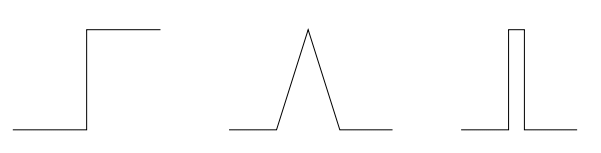
\includegraphics[width=11cm]{Chapiters/Chapiter_01/Pictures/Differents-types-de-contours-marche-descalier-toit-et-pointe.png}
    \caption{image caption.}
    \label{}
\end{figure}

\section{Conclusion}
Sed blandit, diam ut mollis vehicula, tortor mi efficitur dui, quis suscipit mauris velit quis urna. Mauris et ullamcorper augue. Suspendisse nulla est, elementum quis leo a, faucibus convallis lorem. Suspendisse tempor consequat tortor. Maecenas ornare non felis non mattis. Aenean facilisis convallis nisi. Duis mollis nisl vitae aliquam malesuada. Vestibulum eu egestas neque. Fusce ac justo risus. Pellentesque tempus eros non rhoncus condimentum. Aenean pulvinar tristique orci feugiat bibendum. Donec suscipit sem nec massa ultricies tristique sed at tortor. Nulla facilisi. Morbi ut arcu consectetur, hendrerit odio nec, ornare urna. Nunc ac feugiat orci, eget auctor sapien.
      




    \chapter{Deep Learning}
\lhead{\textit{Chapitre \thechapter}}
\rhead{\textit{Deep Learning}}
\section{Introduction}
Lorem ipsum dolor sit amet, consectetur adipiscing elit. Curabitur a ullamcorper purus, sit amet cursus turpis. Nullam ipsum nibh, imperdiet vitae hendrerit et, porta sit amet lorem. In eu sem viverra, condimentum enim ac, congue dui. Quisque quis urna et quam vehicula tristique a a dui. Vestibulum euismod malesuada maximus. Vivamus vel lacinia nisi. Suspendisse ac fermentum ante, vel condimentum odio. Praesent ut nibh tempor, condimentum eros sit amet, scelerisque sapien. Nam ut nisl sit amet risus viverra fringilla quis a sapien. Curabitur id quam nisl. Sed volutpat varius neque eget tempor. Proin eget ultrices magna, ullamcorper ultricies leo. Suspendisse vitae ex sit amet dolor venenatis imperdiet non sit amet turpis. Vestibulum ante ipsum primis in faucibus orci luctus et ultrices posuere cubilia curae; Nulla quis suscipit ipsum. In rhoncus urna a quam eleifend, vitae euismod tellus varius.

\section{Algorithmes de Deep Learning}
Lorem ipsum dolor sit amet, consectetur adipiscing elit. Curabitur a ullamcorper purus, sit amet cursus turpis. Nullam ipsum nibh, imperdiet vitae hendrerit et, porta sit amet lorem. In eu sem viverra, condimentum enim ac, congue dui. Quisque quis urna et quam vehicula tristique a a dui. Vestibulum euismod malesuada maximus. Vivamus vel lacinia nisi. Suspendisse ac fermentum ante, vel condimentum odio. Praesent ut nibh tempor, condimentum eros sit amet, scelerisque sapien. Nam ut nisl sit amet risus viverra fringilla quis a sapien. Curabitur id quam nisl. Sed volutpat varius neque eget tempor. Proin eget ultrices magna, ullamcorper ultricies leo. Suspendisse vitae ex sit amet dolor venenatis imperdiet non sit amet turpis. Vestibulum ante ipsum primis in faucibus orci luctus et ultrices posuere cubilia curae; Nulla quis suscipit ipsum. In rhoncus urna a quam eleifend, vitae euismod tellus varius.

\begin{figure}[htp]
    \centering
    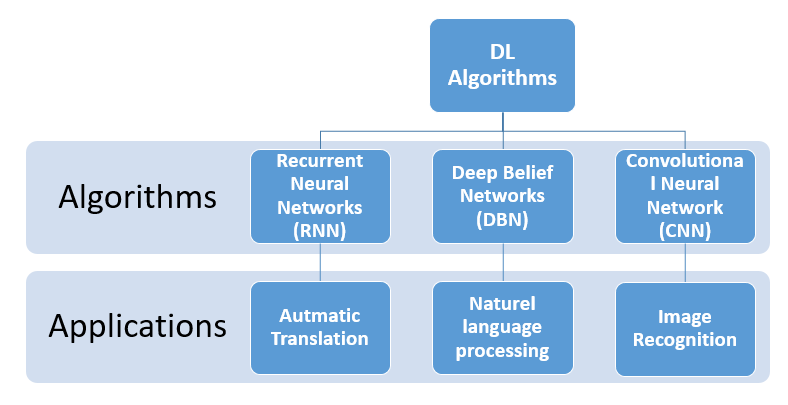
\includegraphics[width=11cm]{Chapiters/Chapiter_02/Pictures/dl_algo.png}
    \caption{Algorithmes de Deep Learning et leur applications.}
    \label{Deep Learning algorithmes et leur applications}
\end{figure}

\section{Conclusion}
Lorem ipsum dolor sit amet, consectetur adipiscing elit. Curabitur a ullamcorper purus, sit amet cursus turpis. Nullam ipsum nibh, imperdiet vitae hendrerit et, porta sit amet lorem. In eu sem viverra, condimentum enim ac, congue dui. Quisque quis urna et quam vehicula tristique a a dui. Vestibulum euismod malesuada maximus. Vivamus vel lacinia nisi. Suspendisse ac fermentum ante, vel condimentum odio. Praesent ut nibh tempor, condimentum eros sit amet, scelerisque sapien. Nam ut nisl sit amet risus viverra fringilla quis a sapien. Curabitur id quam nisl. Sed volutpat varius neque eget tempor. Proin eget ultrices magna, ullamcorper ultricies leo. Suspendisse vitae ex sit amet dolor venenatis imperdiet non sit amet turpis. Vestibulum ante ipsum primis in faucibus orci luctus et ultrices posuere cubilia curae; Nulla quis suscipit ipsum. In rhoncus urna a quam eleifend, vitae euismod tellus varius.
    \chapter{Les Architectures proposées pour la Segmentation d’images Biomédicales}
\lhead{\textit{Chapitre \thechapter}}
\rhead{\textit{Les architectures proposées}}


\section{Introduction}
Lorem ipsum dolor sit amet, consectetur adipiscing elit. Curabitur a ullamcorper purus, sit amet cursus turpis. Nullam ipsum nibh, imperdiet vitae hendrerit et, porta sit amet lorem. In eu sem viverra, condimentum enim ac, congue dui. Quisque quis urna et quam vehicula tristique a a dui. Vestibulum euismod malesuada maximus. Vivamus vel lacinia nisi. Suspendisse ac fermentum ante, vel condimentum odio. Praesent ut nibh tempor, condimentum eros sit amet, scelerisque sapien. Nam ut nisl sit amet risus viverra fringilla quis a sapien. Curabitur id quam nisl. Sed volutpat varius neque eget tempor. Proin eget ultrices magna, ullamcorper ultricies leo. Suspendisse vitae ex sit amet dolor venenatis imperdiet non sit amet turpis. Vestibulum ante ipsum primis in faucibus orci luctus et ultrices posuere cubilia curae; Nulla quis suscipit ipsum. In rhoncus urna a quam eleifend, vitae euismod tellus varius.
\newpage
\section{Description de la solution proposée}
Lorem ipsum dolor sit amet, consectetur adipiscing elit. Curabitur a ullamcorper purus, sit amet cursus turpis. Nullam ipsum nibh, imperdiet vitae hendrerit et, porta sit amet lorem. In eu sem viverra, condimentum enim ac, congue dui. Quisque quis urna et quam vehicula tristique a a dui. Vestibulum euismod malesuada maximus. Vivamus vel lacinia nisi. Suspendisse ac fermentum ante, vel condimentum odio. Praesent ut nibh tempor, condimentum eros sit amet, scelerisque sapien. Nam ut nisl sit amet risus viverra fringilla quis a sapien. Curabitur id quam nisl. Sed volutpat varius neque eget tempor. Proin eget ultrices magna, ullamcorper ultricies leo. Suspendisse vitae ex sit amet dolor venenatis imperdiet non sit amet turpis. Vestibulum ante ipsum primis in faucibus orci luctus et ultrices posuere cubilia curae; Nulla quis suscipit ipsum. In rhoncus urna a quam eleifend, vitae euismod tellus varius.
\vspace{10pt}

\subsection{Architecture U-Net: }
U-Net développée par Zhengxin Zhang et al.
\footnote{U-Net: Convolutional Networks for Biomedical Image Segmentation\newline https://arxiv.org/pdf/1505.04597.pdf} en 2015, était un CNN unique développé pour la segmentation d'images biomédicales,est maintenant devenu un réseau d'encodeur-décodeur très populaire pour la segmentation sémantique il a une architecture UP-Down unique qui a un chemin Contractuel et un chemin Expansif.
\vspace{10pt}
\begin{figure*}[htp]
    \centering
    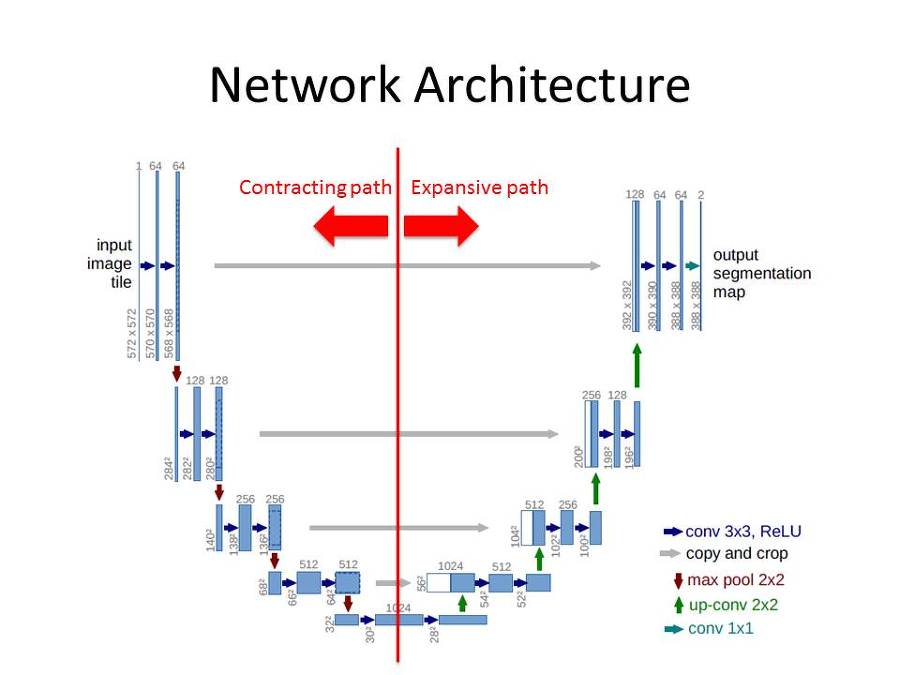
\includegraphics[width=10cm]{Chapiters/Chapiter_03/Pictures/unet.jpg}
    \caption{Architecture U-Net}
    \label{unet}
\end{figure*}
\newpage
\section{Conclusion}
Lorem ipsum dolor sit amet, consectetur adipiscing elit. Curabitur a ullamcorper purus, sit amet cursus turpis. Nullam ipsum nibh, imperdiet vitae hendrerit et, porta sit amet lorem. In eu sem viverra, condimentum enim ac, congue dui. Quisque quis urna et quam vehicula tristique a a dui. Vestibulum euismod malesuada maximus. Vivamus vel lacinia nisi. Suspendisse ac fermentum ante, vel condimentum odio. Praesent ut nibh tempor, condimentum eros sit amet, scelerisque sapien. Nam ut nisl sit amet risus viverra fringilla quis a sapien. Curabitur id quam nisl. Sed volutpat varius neque eget tempor. Proin eget ultrices magna, ullamcorper ultricies leo. Suspendisse vitae ex sit amet dolor venenatis imperdiet non sit amet turpis. Vestibulum ante ipsum primis in faucibus orci luctus et ultrices posuere cubilia curae; Nulla quis suscipit ipsum. In rhoncus urna a quam eleifend, vitae euismod tellus varius. 
    \chapter{Matériels et méthodes }
\lhead{\textit{Chapitre \thechapter}}
\rhead{\textit{Matériels et méthodes }}
\section{Introduction}

Lorem ipsum dolor sit amet, consectetur adipiscing elit. Curabitur a ullamcorper purus, sit amet cursus turpis. Nullam ipsum nibh, imperdiet vitae hendrerit et, porta sit amet lorem. In eu sem viverra, condimentum enim ac, congue dui. Quisque quis urna et quam vehicula tristique a a dui. Vestibulum euismod malesuada maximus. Vivamus vel lacinia nisi. Suspendisse ac fermentum ante, vel condimentum odio. Praesent ut nibh tempor, condimentum eros sit amet, scelerisque sapien. Nam ut nisl sit amet risus viverra fringilla quis a sapien. Curabitur id quam nisl. Sed volutpat varius neque eget tempor. Proin eget ultrices magna, ullamcorper ultricies leo. Suspendisse vitae ex sit amet dolor venenatis imperdiet non sit amet turpis. Vestibulum ante ipsum primis in faucibus orci luctus et ultrices posuere cubilia curae; Nulla quis suscipit ipsum. In rhoncus urna a quam eleifend, vitae euismod tellus varius.

\section{Matériels}
Lorem ipsum dolor sit amet, consectetur adipiscing elit. Curabitur a ullamcorper purus, sit amet cursus turpis. Nullam ipsum nibh, imperdiet vitae hendrerit et, porta sit amet lorem. In eu sem viverra, condimentum enim ac, congue dui. Quisque quis urna et quam vehicula tristique a a dui. Vestibulum euismod malesuada maximus. Vivamus vel lacinia nisi. Suspendisse ac fermentum ante, vel condimentum odio. Praesent ut nibh tempor, condimentum eros sit amet, scelerisque sapien. Nam ut nisl sit amet risus viverra fringilla quis a sapien. Curabitur id quam nisl. Sed volutpat varius neque eget tempor. Proin eget ultrices magna, ullamcorper ultricies leo. Suspendisse vitae ex sit amet dolor venenatis imperdiet non sit amet turpis. Vestibulum ante ipsum primis in faucibus orci luctus et ultrices posuere cubilia curae; Nulla quis suscipit ipsum. In rhoncus urna a quam eleifend, vitae euismod tellus varius.

\subsection{Modèle UNet: }
\begin{figure}[htbp]
\centerline{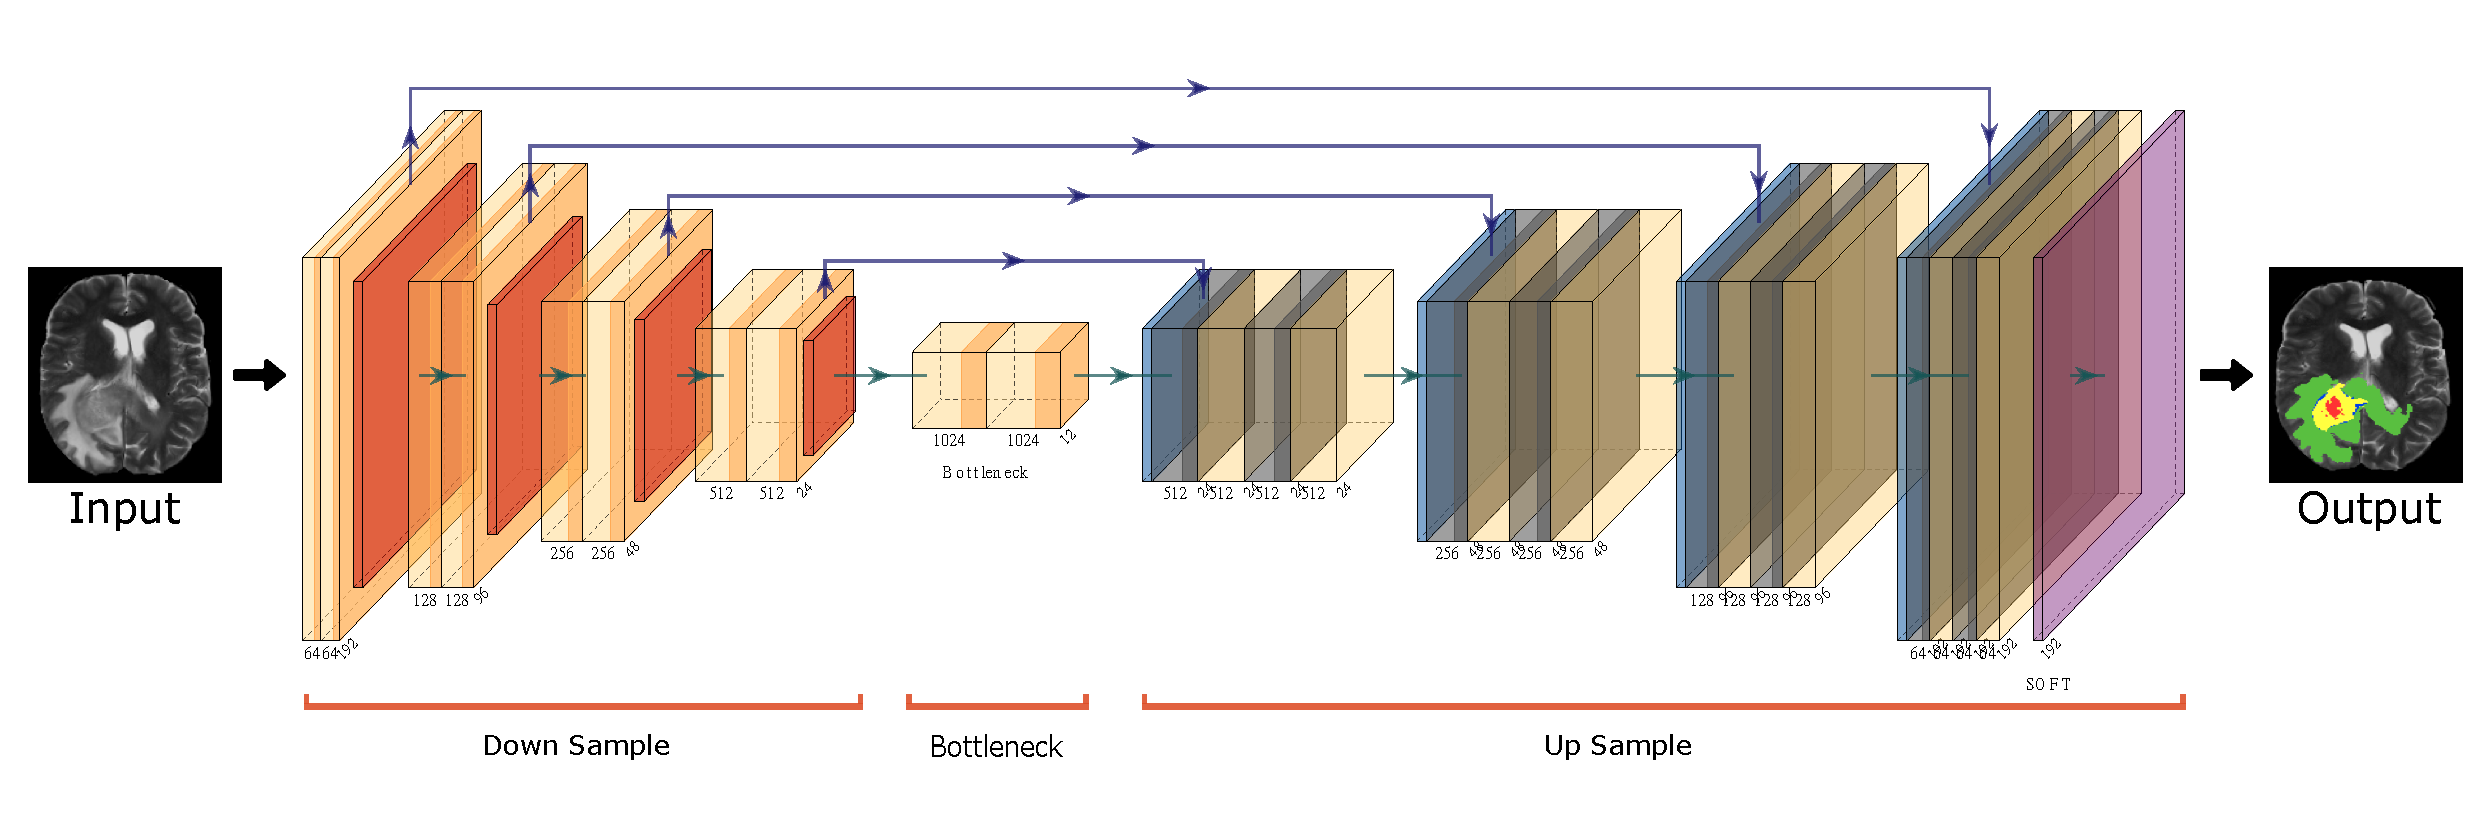
\includegraphics[scale=.4]{Chapiters/Chapiter_04/Pictures/unet.pdf}}
\caption{L'architecure du Modèle U-Net.}
\label{fig}
\end{figure}

\section{Conclusion}
Lorem ipsum dolor sit amet, consectetur adipiscing elit. Curabitur a ullamcorper purus, sit amet cursus turpis. Nullam ipsum nibh, imperdiet vitae hendrerit et, porta sit amet lorem. In eu sem viverra, condimentum enim ac, congue dui. Quisque quis urna et quam vehicula tristique a a dui. Vestibulum euismod malesuada maximus. Vivamus vel lacinia nisi. Suspendisse ac fermentum ante, vel condimentum odio. Praesent ut nibh tempor, condimentum eros sit amet, scelerisque sapien. Nam ut nisl sit amet risus viverra fringilla quis a sapien. Curabitur id quam nisl. Sed volutpat varius neque eget tempor. Proin eget ultrices magna, ullamcorper ultricies leo. Suspendisse vitae ex sit amet dolor venenatis imperdiet non sit amet turpis. Vestibulum ante ipsum primis in faucibus orci luctus et ultrices posuere cubilia curae; Nulla quis suscipit ipsum. In rhoncus urna a quam eleifend, vitae euismod tellus varius.
    \chapter{Réalisation}
\lhead{\textit{Chapitre \thechapter}}
\rhead{\textit{Réalisation}}

\section{Introduction}
Lorem ipsum dolor sit amet, consectetur adipiscing elit. Curabitur a ullamcorper purus, sit amet cursus turpis. Nullam ipsum nibh, imperdiet vitae hendrerit et, porta sit amet lorem. In eu sem viverra, condimentum enim ac, congue dui. Quisque quis urna et quam vehicula tristique a a dui. Vestibulum euismod malesuada maximus. Vivamus vel lacinia nisi. Suspendisse ac fermentum ante, vel condimentum odio. Praesent ut nibh tempor, condimentum eros sit amet, scelerisque sapien. Nam ut nisl sit amet risus viverra fringilla quis a sapien. Curabitur id quam nisl. Sed volutpat varius neque eget tempor. Proin eget ultrices magna, ullamcorper ultricies leo. Suspendisse vitae ex sit amet dolor venenatis imperdiet non sit amet turpis. Vestibulum ante ipsum primis in faucibus orci luctus et ultrices posuere cubilia curae; Nulla quis suscipit ipsum. In rhoncus urna a quam eleifend, vitae euismod tellus varius.
\section{Les outils de développement}
\subsection{Langage de programmation}
Le langage de programmation choisi pour notre méthode présentée précédemment s'est concentré sur le langage python

\textbf{Python:}

Python\footnote{https://www.python.org/}est un langage de programmation puissant et facile à apprendre. Il a des données de haut niveau
structures et permet une approche simple mais efficace de la programmation orientée objet.

Python est un langage de programmation interprété, un langage de script et est un peu lent
par rapport à d'autres langages compilés en C ou C++ pour faire des calculs. Offres Python
plusieurs bibliothèques (packages) pour le traitement des données, les calculs matriciels, l'analyse et les données
visualisation. Pour le Deep Learning, python a des environnements de travail comme caffe, tensorow,
keras, pytorch. Ces environnements de travail sont très utiles car ils permettent de
gérer l'algorithme de rétropropagation pour les grands réseaux de neurones, les CNN, les U-net, etc.
Ils assurent également la parallélisation des calculs sur le GPU. 

Le choix de ce langage présente les avantages suivants :
\begin{itemize}
\item C'est totalement gratuit.
\item  Il est facile à apprendre, lire, comprendre, utiliser et écrire.
\item Il fonctionne sur tous les principaux systèmes d'exploitation et plates-formes informatiques.
\end{itemize}


\subsection{Environnement de développement}
Tout entraînement du réseau de neurones nécessite une forte puissance de calcul. Notre méthode est
basée sur un réseau convolutif profond, qui implique un grand nombre de points à entraîner.
La formation sur le PC portable aurait également pris beaucoup de temps. Nous avons utilisé Google Colab et Amazon Sagemaker studio.\newline

$\blacksquare$ \textbf{ Google Colab:}
Google Colaboratory ou Colab, un outil Google simple et gratuit pour vous initier au Deep Learning ou collaborer avec vos collègues sur des projets en science des données \cite{gcolab}. 
  
Colab permet :
\begin{itemize}
\item de développer des applications en Deep Learning en utilisant des bibliothèques Python populaires telles que Keras, TensorFlow, PyTorch et OpenCV.
\item  Il est facile à apprendre, lire, comprendre, utiliser et écrire.
\item d’utiliser un environnement de développement (Jupyter Notebook) qui ne nécessite aucune configuration.
Mais la fonctionnalité qui distingue Colab des autres services est l’accès à un processeur graphique GPU, totalement gratuitement.
\end{itemize}

$\blacksquare$ \textbf{ Amazon Sagemaker studio:}

Amazon SageMaker est un service entièrement géré permettant aux développeurs et aux spécialistes des données de créer, former et déployer rapidement et facilement des modèles de machine learning \cite{amazonsm}.

\subsection{Bibliothèques utilisées :}
Plusieurs bibliothèques ont été utilisées. Dans notre travail, nous avons besoin des bibliothèques suivantes :

\begin{enumerate}
    \item \textbf{TensorFlow :}

TensorFlow\footnote{https://www.tensorflow.org/} est une plate-forme open source de bout en bout pour l'apprentissage automatique. Il dispose d'un écosystème complet et flexible d'outils, des bibliothèques et des ressources communautaires qui permet aux chercheurs de poussez l'état de l'art en matière de ML et les développeurs créent et déploient facilement des applications basées sur ML.

De nombreuses entreprises utilisent TensorFlow telles que Google, Twitter, Intel et Coca-Cola, il est très apprécié pour ses nombreux bienfaits que nous listons ci-dessous :
\begin{itemize}

\item Multi-platform (Linux, Mac OS, Windows and even Android and iOS).

\item APIs in Python, C ++, Java.

\item Documentation extrêmement bien fournie avec de nombreux exemples et tutoriels.

\end{itemize}
\item \textbf{Keras}

Keras\footnote{https://keras.io/} est une API d'apprentissage en profondeur écrite en Python, s'exécutant au-dessus de l'apprentissage automatique plate-forme TensorFlow.
\item \textbf{SimpleITK} 

SimpleITK\footnote{https://simpleitk.org/} est une interface open source simplifiée de la boîte à outils de segmentation et d'enregistrement Insight. La bibliothèque d'analyse d'images SimpleITK est disponible dans plusieurs langages de programmation, notamment C ++, Python, R...

\item \textbf{Matplotlib}
Matplotlib\footnote{https://matplotlib.org/} est une bibliothèque de suivi Python 2D qui produit des images de qualité publication dans
divers formats papier et environnements interactifs sur toutes les plateformes.

\item \textbf{NumPy}
NumPy\footnote{https://numpy.org/} est une bibliothèque pour le langage de programmation Python, a destinée à manipuler des matrices ou tableaux multidimensionnels, ainsi qu'une grande collection des fonctions mathématiques de haut niveau pour opérer sur ces tableaux.

\item \textbf{Pandas}
Pandas\footnote{https://pandas.pydata.org/}est une analyse de données open source rapide, puissante, flexible et facile à utiliser.

\item \textbf{Scikit-learn}

Scikit-learn\footnote{https://scikit-learn.org/} est une bibliothèque en Python qui fournit de nombreux algorithmes d'apprentissage. Il comprend des fonctions pour l'estimation de la régression logistique, des algorithmes de classification et des vecteurs de support Machines.
\end{enumerate}



\section{Conclusion}
Lorem ipsum dolor sit amet, consectetur adipiscing elit. Curabitur a ullamcorper purus, sit amet cursus turpis. Nullam ipsum nibh, imperdiet vitae hendrerit et, porta sit amet lorem. In eu sem viverra, condimentum enim ac, congue dui. Quisque quis urna et quam vehicula tristique a a dui. Vestibulum euismod malesuada maximus. Vivamus vel lacinia nisi. Suspendisse ac fermentum ante, vel condimentum odio. Praesent ut nibh tempor, condimentum eros sit amet, scelerisque sapien. Nam ut nisl sit amet risus viverra fringilla quis a sapien. Curabitur id quam nisl. Sed volutpat varius neque eget tempor. Proin eget ultrices magna, ullamcorper ultricies leo. Suspendisse vitae ex sit amet dolor venenatis imperdiet non sit amet turpis. Vestibulum ante ipsum primis in faucibus orci luctus et ultrices posuere cubilia curae; Nulla quis suscipit ipsum. In rhoncus urna a quam eleifend, vitae euismod tellus varius.



    \chapter*{Conclusion générale}
\addcontentsline{toc}{chapter}{Conclusion générale}
\lhead{}
\rhead{\textit{Conclusion générale}}
Lorem ipsum dolor sit amet, consectetur adipiscing elit. Curabitur a ullamcorper purus, sit amet cursus turpis. Nullam ipsum nibh, imperdiet vitae hendrerit et, porta sit amet lorem. In eu sem viverra, condimentum enim ac, congue dui. Quisque quis urna et quam vehicula tristique a a dui. Vestibulum euismod malesuada maximus. Vivamus vel lacinia nisi. Suspendisse ac fermentum ante, vel condimentum odio. Praesent ut nibh tempor, condimentum eros sit amet, scelerisque sapien. Nam ut nisl sit amet risus viverra fringilla quis a sapien. Curabitur id quam nisl. Sed volutpat varius neque eget tempor. Proin eget ultrices magna, ullamcorper ultricies leo. Suspendisse vitae ex sit amet dolor venenatis imperdiet non sit amet turpis. Vestibulum ante ipsum primis in faucibus orci luctus et ultrices posuere cubilia curae; Nulla quis suscipit ipsum. In rhoncus urna a quam eleifend, vitae euismod tellus varius.

Lorem ipsum dolor sit amet, consectetur adipiscing elit. Curabitur a ullamcorper purus, sit amet cursus turpis. Nullam ipsum nibh, imperdiet vitae hendrerit et, porta sit amet lorem. In eu sem viverra, condimentum enim ac, congue dui. Quisque quis urna et quam vehicula tristique a a dui. Vestibulum euismod malesuada maximus. Vivamus vel lacinia nisi. Suspendisse ac fermentum ante, vel condimentum odio. Praesent ut nibh tempor, condimentum eros sit amet, scelerisque sapien. Nam ut nisl sit amet risus viverra fringilla quis a sapien. Curabitur id quam nisl. Sed volutpat varius neque eget tempor. Proin eget ultrices magna, ullamcorper ultricies leo. Suspendisse vitae ex sit amet dolor venenatis imperdiet non sit amet turpis. Vestibulum ante ipsum primis in faucibus orci luctus et ultrices posuere cubilia curae; Nulla quis suscipit ipsum. In rhoncus urna a quam eleifend, vitae euismod tellus varius.
    \clearpage
    \newpage
    \addcontentsline{toc}{chapter}{Bibliographie}
    \printbibliography
    

    
    
    \end{document}
